\documentclass{beamer}
\usepackage{amsmath}
\usepackage{graphicx}
\usepackage{hyperref}
\usetheme{Madrid}
\usecolortheme{default}

\setbeamertemplate{bibliography item}{\insertbiblabel}


\newcommand{\mbeq}{\overset{!}{=}}

\title[Master's Seminar]
{Defaultable LIBOR Market Models for Loan Valuation and their Implementation}

\subtitle{Master's Thesis}

\author[M. Parhofer] % (optional, for multiple authors)
{Markus Parhofer}

\institute[LMU] % (optional)
{
	Supervision:\\Prof. Dr. Christian Fries and Prof. Dr. Andrea Mazzon 
}

\date[December 14th, 2023] % (optional)
{December 14th, 2023}

\definecolor{lmugreen}{RGB}{0,136,58}
\definecolor{lmugreenmid}{RGB}{51,160,97}
\definecolor{lmugreenlight}{RGB}{102,184,137}

\setbeamercolor{titlelike}{bg=lmugreen}
\setbeamerfont{title}{series=\bfseries}
\setbeamercolor*{palette tertiary}{bg=lmugreen, fg=white}
\setbeamercolor*{palette secondary}{bg=lmugreenmid, fg=white}
\setbeamercolor*{palette primary}{bg=lmugreenlight, fg=white}

\begin{document}
	
	\frame{\titlepage}
	
	\begin{frame}
		\frametitle{Table of Contents}
		\tableofcontents
	\end{frame}
	
	\section{General setting: LIBOR Market Model}\label{sectGeneral}
	
	\begin{frame}
		\frametitle{\nameref{sectGeneral}}
		\tableofcontents[ 
		currentsection, 
		sectionstyle=show/shaded, 
		subsectionstyle=show/shaded, 
		] 
	\end{frame}
	
	\begin{frame}
		\frametitle{Framework}
		
		During the whole talk we make a few assumptions:
		\begin{itemize}
			\item The market is arbitrage free and complete.
			\item We work in the setting of $(\Omega, \mathcal{F}, (\mathcal{F}_t)_{t\in \left[0,T\right]}, \mathbb{Q}^B)$.
			\item $B(t)$ is a numeraire that is $\mathcal{F}_t$-measurable. We mainly consider the Spot measure.
			\item $\mathbb{Q}^B$ is the martingale measure corresponding to the numeraire.
			\item This means that all traded assets discounted by $B(t)$ are martingales w.r.t. $\mathbb{Q}^B$ (see \cite{fima2Lecture}).
			\item We have a time tenor $0 = T_0 < ... < T_N = T$ that splits $[0,T]$.
			%
			%\item Notation: while we will mostly write $\mu$ and $\lambda$ as drift and diffusion terms in SDEs note that they can and in most cases are dependent on t and on their SDE solution 
		\end{itemize}
		
	\end{frame}
	
	\begin{frame}{General Setting}
		We are in the setting of a general LIBOR market model:\\
		\begin{itemize}
			\item We have $N$ zero coupon bonds with price $P(t; T_i)$, where $P(T_i;T_i) = 1$.
			\item These are traded assets $\Rightarrow$ discounted price processes are martingales.
			\item We derive simple forward rates for the tenor:
			
			\[
			L_i(t) := L(t; T_i, T_{i+1}) = \frac{1}{T_{i+1} - 	T_i}\left(\frac{P(t;T_i)}{P(t;T_{i+1})} - 1\right)
			\]
			\par
			\item ... and their SDE:
			\[
			dL_i(t) = \mu _i dt + \sum_{k=0}^{M}\lambda _{i,k}dW^k_t,
			\]
		\end{itemize}
		where $\lambda_{i, k}$ are factor loadings (we assume $M + 1$ factors), $W_k$ are $M+1$ independent brownian motions and $L=(L_0, ..., L_{N-1})^T$.
	\end{frame}
	
	\begin{frame}{The Numeraire: Spot measure}
		The choice of numeraire influences the SDE, i.e. the drift $\mu_k$:\\
		\begin{itemize}
			\item Under the \textbf{Spot} measure we specify the numeraire:
			\[
			B(t) := P(t; T_{m\left( t\right)  + 1})\prod_{j=0}^{m\left( t\right) }(1+L_j(T_j)\Delta T_j)
			\]
			\item The drift is then:
			\[
			\mu_i(t, L(t)) = \sum_{j=m\left( t\right)  + 1}^{i} \lambda_{i}\lambda_{j}^T  \frac{\Delta T_j}{1 + \Delta T_j \;L_j(t)}
			\]
		
		\end{itemize}
			where $m(t) = \max(i \in \{0, ..., N-1\} | T_i \le t)$.
			Note that $\lambda_i \lambda^T_j = |\sigma_{i}| |\sigma_{j}| \rho_{i,j}$ is the "covariance" between the $i$-th and $j$-th LIBOR rate.
	\end{frame}
	
	\begin{frame}{The Numeraire: Terminal measure}
		\begin{itemize}
			\item Under the \textbf{Terminal} measure we have the numeraire:
			\[
			B(t) := P(t; T_{N})
			\]
			\item The drift is then:
			\[
			\mu_i(t, L(t)) = - \sum_{j=i+1}^{N-1} \lambda_{i}\lambda_{j}^T  \frac{\Delta T_j}{1 + \Delta T_j \;L_j(t)}
			\]
			
		\end{itemize}
		
		For a proof of these results see \cite{FriesBook} and \cite{fima3Lecture}.
	\end{frame}
	
	\section{Defaultable LIBOR Market Model}\label{sectDLMM}
	
	\begin{frame}
		\frametitle{\nameref{sectDLMM}}
		\tableofcontents[ 
		currentsection, 
		sectionstyle=show/shaded, 
		subsectionstyle=show/shaded, 
		] 
	\end{frame}

	\begin{frame}
		\frametitle{Defaultable Bonds}
		Let us extend this model:
		\begin{itemize}
			\item We now assume an additional set of \textbf{defaultable} zero coupon bonds $P^d(t;T_i)$ with the same maturities.
			\item Their payoff is:
			\[P^d(T_i;T_i) = \mathbf{1}_{\{\tau > T_i\}},\]
			\item $\tau(\omega)$ denotes the (stochastic) default time. 
			%\item It is a stopping time with respect to our filtration $(\mathcal{F}_t)_{t\in [0,T_N]}$.
			\item Lets split the defaultable bond into a continuous and discontinuous part:
			\[P^d(t;T_i) = P^{d,*}(t;T_i)(1 - J(t))\quad J(t):= \mathbf{1}_{\{\tau \le t\}}\]
			\item where $P^{d,*}$ denotes the defaultable zero coupon bond conditional on predefault (see also \cite{friesDLMM}).
		\end{itemize}
	\end{frame}
	
	\begin{frame}
		\frametitle{Defaultable Libor rates}
		\begin{itemize}
			\item We can also define LIBOR rates on the defaultable bonds conditional on predefault:
		\[L^{d}_i(t) := L^{d}(t; T_i, T_{i+1}) = \frac{1}{ \Delta T_i}\left( \frac{P^{d,*}(t; T_i)}{P^{d,*}(t; T_{i+1})} - 1\right) .\]
		\item Assume $L^d$ is driven by $M^d - M$ extra factors
		\item With factor loadings \(\lambda^d_i = (\lambda^d_{i \, 0}, ..., \lambda^d_{i \, M^d})\) for component \(i\) the defaultable LIBOR rates then follow the dynamic:
		\[dL^d_i(t) = \mu_i^ddt + \sum_{k=0}^{M^d}\lambda^d_{i \, k} dW^k_t,\]
		
	\end{itemize}
	where we again need to derive \(\mu^d(t, L^d(t))\).
	\end{frame}
	
	\begin{frame}
	\frametitle{$\mu^d$ under the Spot measure}
	It turns out the drift term of the defaultable LIBORs under the Spot measure looks very similar to those of the non defaultable ones:
	\[
	\mu^d_i(t, L^d) = \sum_{j=m\left( t\right)  + 1}^{i} \lambda^d_{i}\lambda^{d \, T}_{j}  \frac{\Delta T_j}{1 + \Delta T_j \; L^d_j(t)}.
	\]
	Let us take a peek at an outline of the proof.
	\end{frame}
	
	\begin{frame}
		\frametitle{Outline of the proof}
		
		\begin{itemize}
			\item We first realize $P^d(t; T_i)$ and hence also $L^d_i(t) P^d(t;T_{i+1})$ are traded assets and thus discounted with $B(t)$ must be martingales w.r.t $\mathbb{Q}^B$.
			\item We use the product rule to see:
			\begin{align*}
			d(L^d_i(t)\frac{P^d(t;T_{i+1})}{B(t)}) = &\frac{P^d(t;T_{i+1})}{B(t)} dL^d_i(t) + L^d_i(t) d\frac{P^d(t;T_{i+1})}{B(t)}\\
			& + dL^d_i(t) d\frac{P^d(t;T_{i+1})}{B(t)}
			\end{align*}
			\item Comparing drifts we find:
			\[\frac{P^d(t;T_{i+1})}{B(t)} \mu^d dt = -dL^d_i(t) d\frac{P^d(t;T_{i+1})}{B(t)}\]
		\end{itemize}
		
	\end{frame}
	
	\begin{frame}
		\frametitle{Outline of the proof}
		\begin{itemize}
			\item We have
			\(
				P^d(t;T_{i+1}) = P^d(t;T_{m(t)+1}) \prod_{j=m\left( t\right) + 1}^{i}(1 + \Delta T_j L^d_{j})^{-1}
			\)
			\item We assume $P^{(d)}(t; T_{m(t)+1})$ have no diffusion, hence:
			\begin{align*}
				d\frac{P^d(t;T_{m(t)+1})}{P(t;T_{m(t)+1})} = (...)dt - \frac{P^{d,*}(t;T_{m(t)+1})}{P(t;T_{m(t)+1})}dJ(t),
			\end{align*}
			\item We get (note $dX dJ = 0$ for all Itô processes $X$):
			\begin{align*}
				d\frac{P^d(t;T_{i+1})}{B(t)} = (...) dt &- \frac{P^d(t;T_{i+1})}{B(t)} \sum_{k=0}^{M^d}\sum_{j=m(t)+1}^{i}\frac{\Delta T_j \lambda_{j \, k}}{1+\Delta T_j L^d_j} dW^k_t \\
				&- \frac{P^{d,*}(t;T_{i+1})}{B(t)}dJ(t).
			\end{align*}
			\item Which concludes the proof.
		\end{itemize}
		
	\end{frame}
	
	\begin{frame}
		\frametitle{Spreads}
		A spread is the difference between defaultable and non defaultable forward rates (i.e. $S_i = L^d_i - L_i$).
		\begin{itemize}
			\item The general dynamic for the spread is then:
			\begin{align*}
			dS_i = (\mu^d(t, L_i^d)- \mu(t, L_i))dt + \sum_{k=0}^{M^d}(\lambda^d_{i \, k} - \lambda_{i \, k} \mathbf{1}_{k < M}) dW^k_t
			\end{align*}
			\item This does not imply positive spread values.
			\item A negative spread would constitute an arbitrage possibility.
			\item Hence through the choice of $\lambda^d $ we need to generate a dynamic for $S$ that \textbf{guarantees positivity}.
		\end{itemize}
	\end{frame}
	
	\begin{frame}
		\frametitle{Diffusions generating Log-Normal Spreads}
		Let us choose as factor loadings
		\begin{align*}
		\lambda_{i \, k}^d &= \dfrac{1+L^d_i(t)\Delta T_i}{1+L_i(t)\Delta T_i} \lambda_{i \, k}
		\quad & \text{ if } k \leq M \text{, and}\\
		\lambda_{i \, k}^d &= (L^d_i(t) - L_i(t)) f_{i \, k}
		&\text{ if } M < k \leq M^d \text{,}
		\end{align*}
		where $f_{i \, k}$ are free parameters.\\
		This will yield a log normal spread dynamic (I challenge you to try proving this yourself ;), otherwise a proof can be found in \cite{friesDLMM}):
		\[dS_i = S_i\mu^Sdt + S_i \sum_{k=0}^{M^d}\lambda^S_{i k}dW^k_t\]
	\end{frame}
	
	\begin{frame}
		\frametitle{Survival Probability}
		We can now construct the survival probabilities:
		\begin{itemize}
			\item At the tenor times $T_i$ the numeraire under the Spot measure is $\mathcal{F}_{T_{i-1}}$ measurable.
			\item This implies the one step survival probability:
			\[\mathbb{Q}^B(\{\tau > T_{i+1} \;|\;\tau > T_i\})(\omega) = \frac{P^{d,*}(T_i;T_{i+1})}{P(T_i;T_{i+1})}\]
			\item Since we assume $\mathbb{Q}^B(\tau > T_0) = 1$, Bayes-rule implies:
			\[\mathbb{Q}^B(\tau > T_i)(\omega) = \prod_{k=0}^{i-1}\frac{P^{d,*}(T_k;T_{k+1})}{P(T_k;T_{k+1})} = \frac{B(T_i)}{B^d(T_i)},\]
		\end{itemize}
		where \(B^d(t) := P^{d,*}(t;T_{m(t)+1})\prod_{k=0}^{m(t)}(1+L^d_k(T_k)\Delta T_k)\)
	\end{frame}
	
	\section{Implementation}\label{Implementation}
	
	\begin{frame}
		\frametitle{\nameref{Implementation}}
		\tableofcontents[ 
		currentsection, 
		sectionstyle=show/shaded, 
		subsectionstyle=show/shaded, 
		] 
	\end{frame}
	
	\begin{frame}
		\frametitle{Introduction to Finmath Library}
		
		The Finmath Library is an object oriented Java library that is open source and was built by Prof. Dr. Fries \cite{finmathWebsite}.\\
		It strongly follows the concepts of \textbf{abstraction}, \textbf{high cohesion} and \textbf{single responsibility principle}.
		\begin{itemize}
			\item \textbf{Abstraction}: take in interfaces instead of classes.
			\item \textbf{High Cohesion}: closely related constructs should be given in the same module, object or function.
			\item \textbf{Single Responsibility Principle}: each part of the program should have a well defined and single responsibility.
		\end{itemize}
		
	\end{frame}
	
	\begin{frame}
		\frametitle{Implementation of a Defaultable LIBOR Market Model}
		In the diagram we can see how we use these concepts to create a flexible DefaultableLIBORMarketModel:
		\begin{figure}
			\centering
			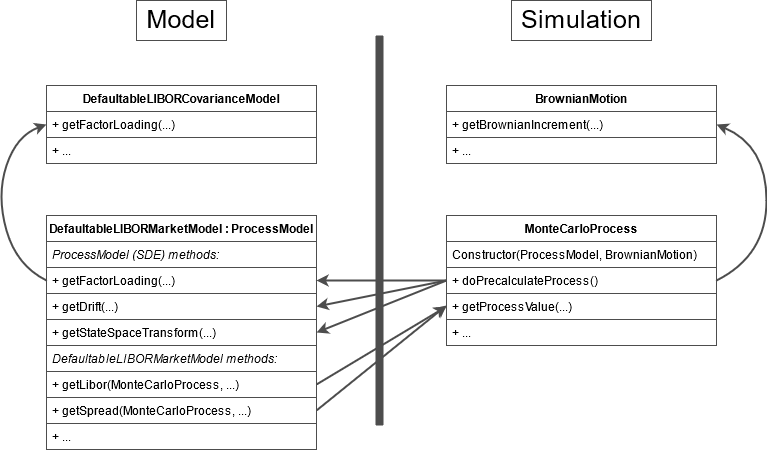
\includegraphics[width=0.7\linewidth]{ClassDiagramDefaultableLIBORMarketModel}
			\caption{Separation of Model and Simulation}
			\label{fig:classdiag}
		\end{figure}
		
	\end{frame}
	\begin{frame}
		\frametitle{Discretization Schemes}
		\begin{itemize}
			\item Euler scheme:
			\[\tilde{X}_{t_{i+1}} = \mu^X(t_i, \tilde{X}_{t_i}) \Delta t_i + \lambda^X(t_i, \tilde{X}_{t_i}) \cdot \Delta W_{t_i}\]
			\item Milstein scheme:
			\begin{align*}
			\tilde{X}_{t_{i+1}} = &\mu^X(t_i, \tilde{X}_{t_i}) \Delta t_i + \lambda^X(t_i, \tilde{X}_{t_i}) \cdot \Delta W_{t_i}\\
			& + \frac{1}{2}\lambda^X(t_i, \tilde{X}_{t_i})  \frac{\partial \lambda^X}{\partial x}(t_i, \tilde{X}_{t_i})((\Delta W_{t_i})^2 - \Delta t_i)
			\end{align*}
			\item State-space adjusted Euler Scheme for a process $X_t = f(Y_t)$:
			\begin{enumerate}
				\item Approximate $Y_t$ by Euler scheme $\tilde{Y}_{t_i}$
				\item Set $\tilde{X}_{t_i} = f(\tilde{Y}_{t_i})$
			\end{enumerate}
		\end{itemize}
		The schemes are all described and analyzed in \cite{kloedenSchemes}, \cite{FriesBook} and \cite{finmathWebsite}.
	\end{frame}
	
	\begin{frame}
		\frametitle{Problems with Schemes}
		
		\begin{figure}
			\centering
			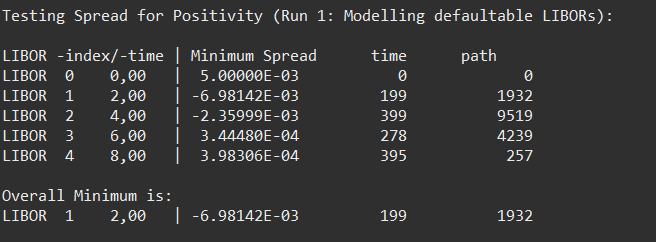
\includegraphics[width=0.7\linewidth]{VorstellungPics/ProblemsEuler}
			\caption{Minimum Path Values Euler Scheme}
			\label{fig:problemseuler}
		\end{figure}
		
		
	\end{frame}
	
	\begin{frame}
		\frametitle{Problems with Schemes}
		
		\begin{figure}
			\begin{minipage}[c]{0.4\linewidth}
				\centering
				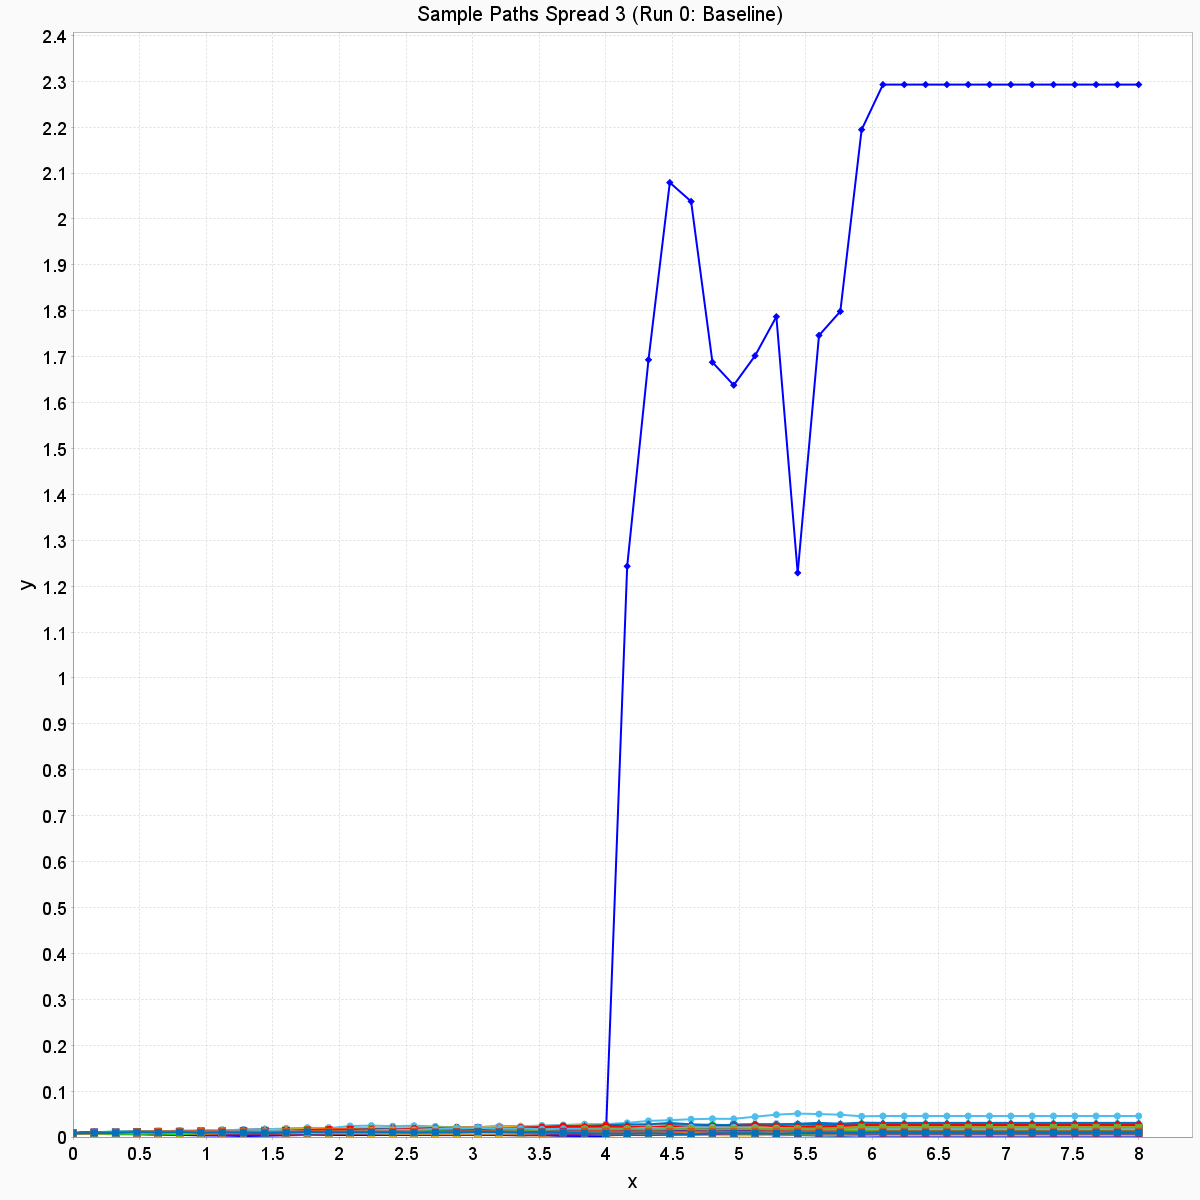
\includegraphics[height=0.6\textheight]{VorstellungPics/ProblemsEULERFuncPaths}
				\caption{Paths Functional Euler Scheme}
				\label{fig:problemseulerfuncpaths}
			\end{minipage}
			\hfill
			\begin{minipage}[c]{0.4\linewidth}
				\centering
				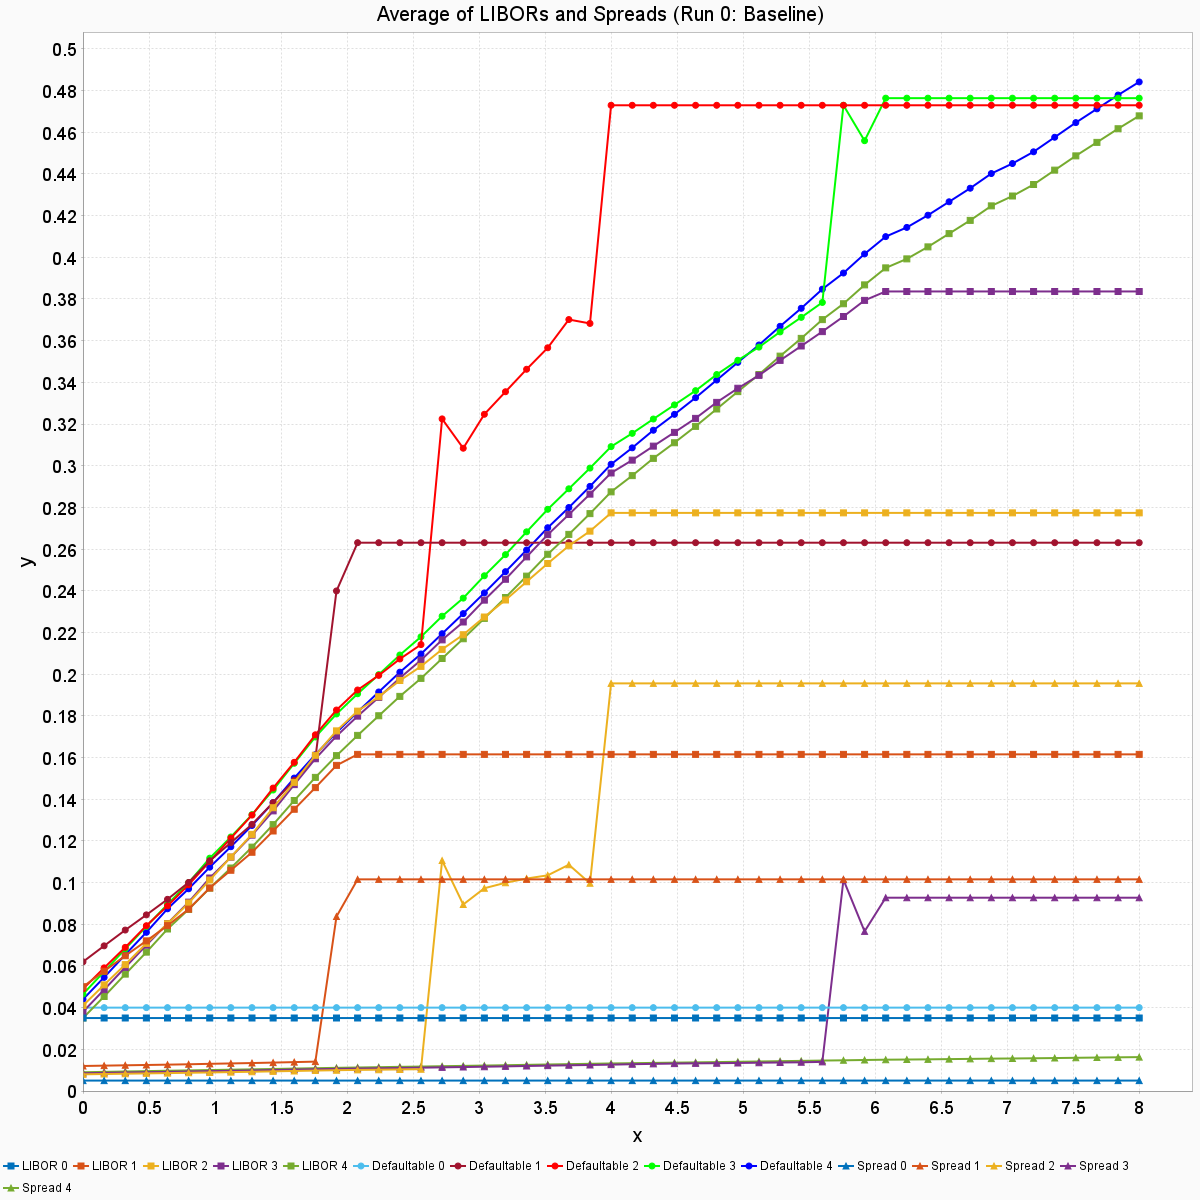
\includegraphics[width=0.9\linewidth]{VorstellungPics/ProblemsEULERFuncAv}
				\caption{Averages Functional Euler Scheme}
				\label{fig:problemseulerfuncav}
			\end{minipage}%
		\end{figure}
		
%		\begin{figure}
%			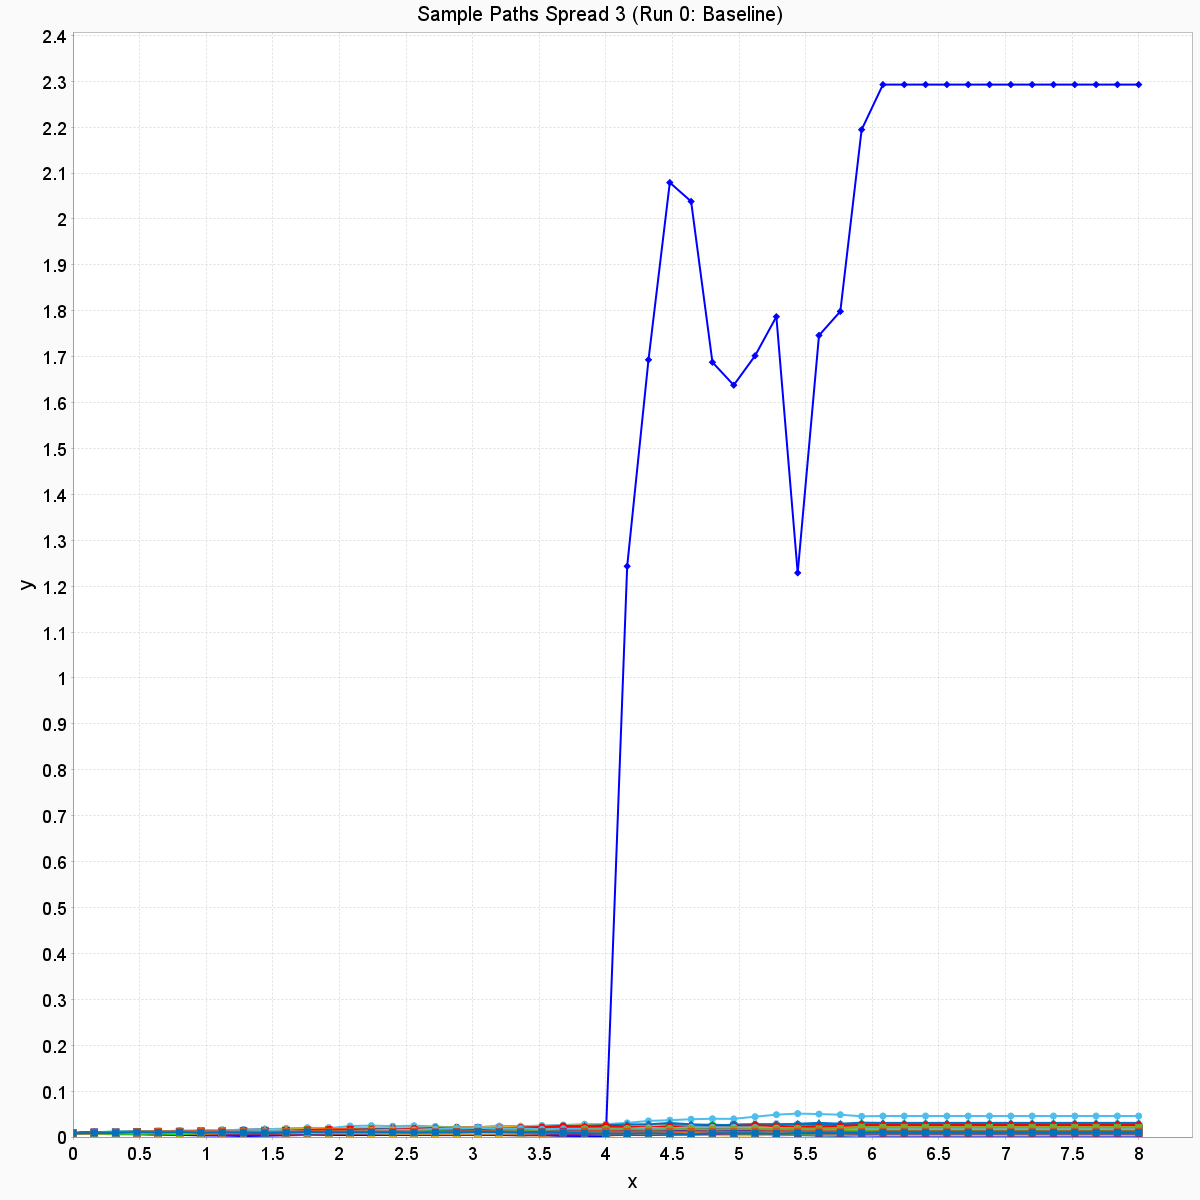
\includegraphics[height=0.6\textheight]{VorstellungPics/ProblemsEULERFuncPaths}
%			\caption{Paths Functional Euler Scheme}
%			\label{fig:problemseulerfuncpaths}
%		\end{figure}
%		\begin{figure}
%			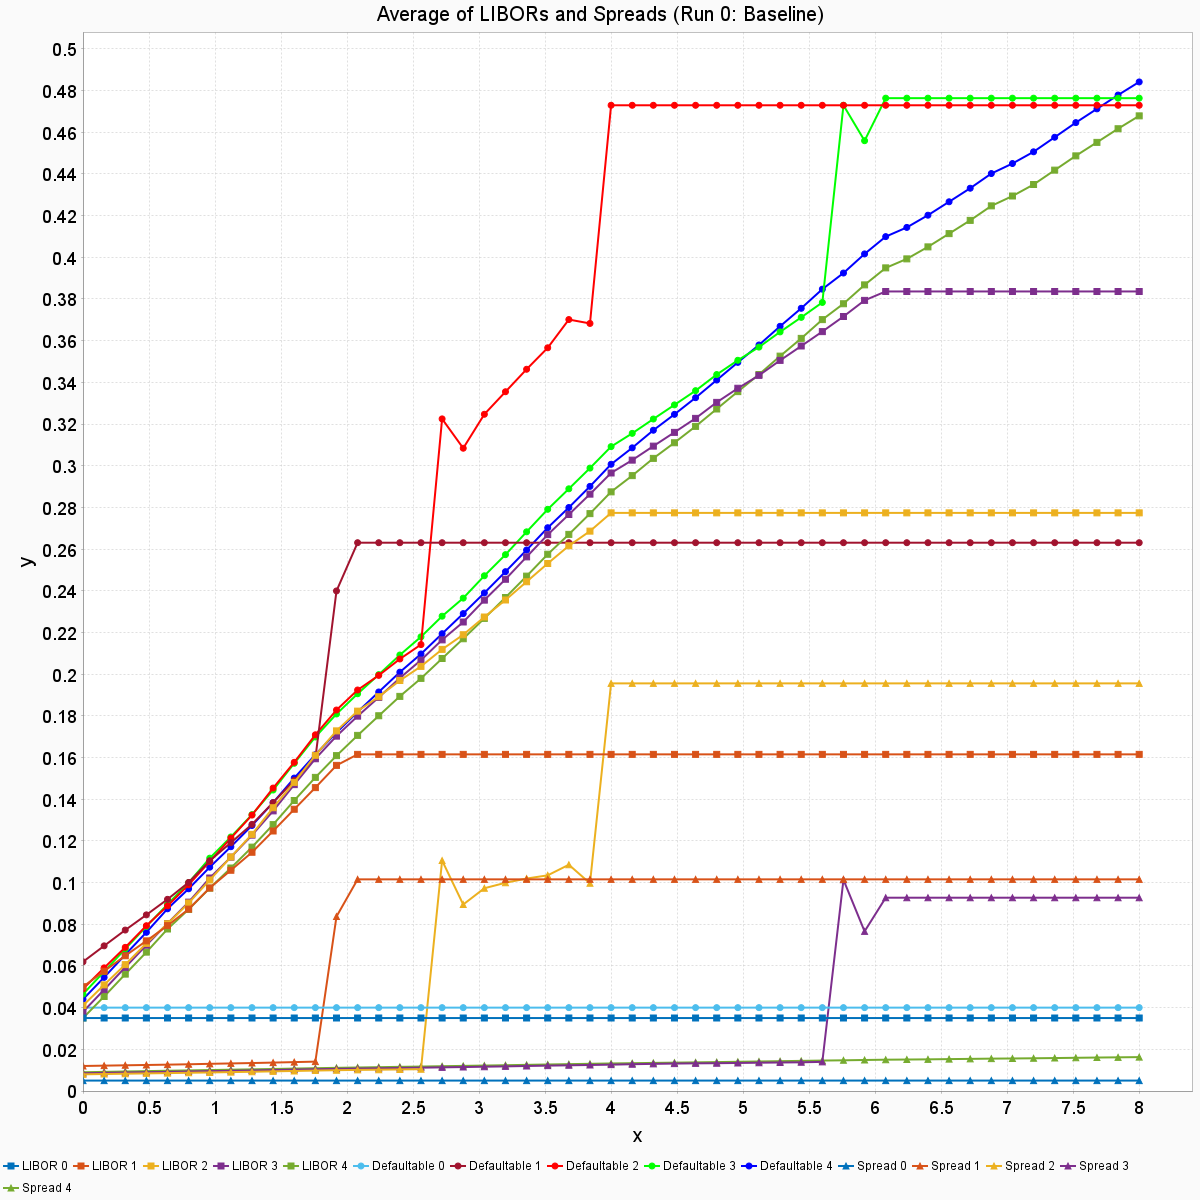
\includegraphics[height=0.6\textheight]{VorstellungPics/ProblemsEULERFuncAv}
%			\caption{Averages Functional Euler Scheme}
%			\label{fig:problemseulerfuncav}
%		\end{figure}
%		
	\end{frame}
	
	\begin{frame}
		\frametitle{Results}
	\begin{figure}
		\centering
		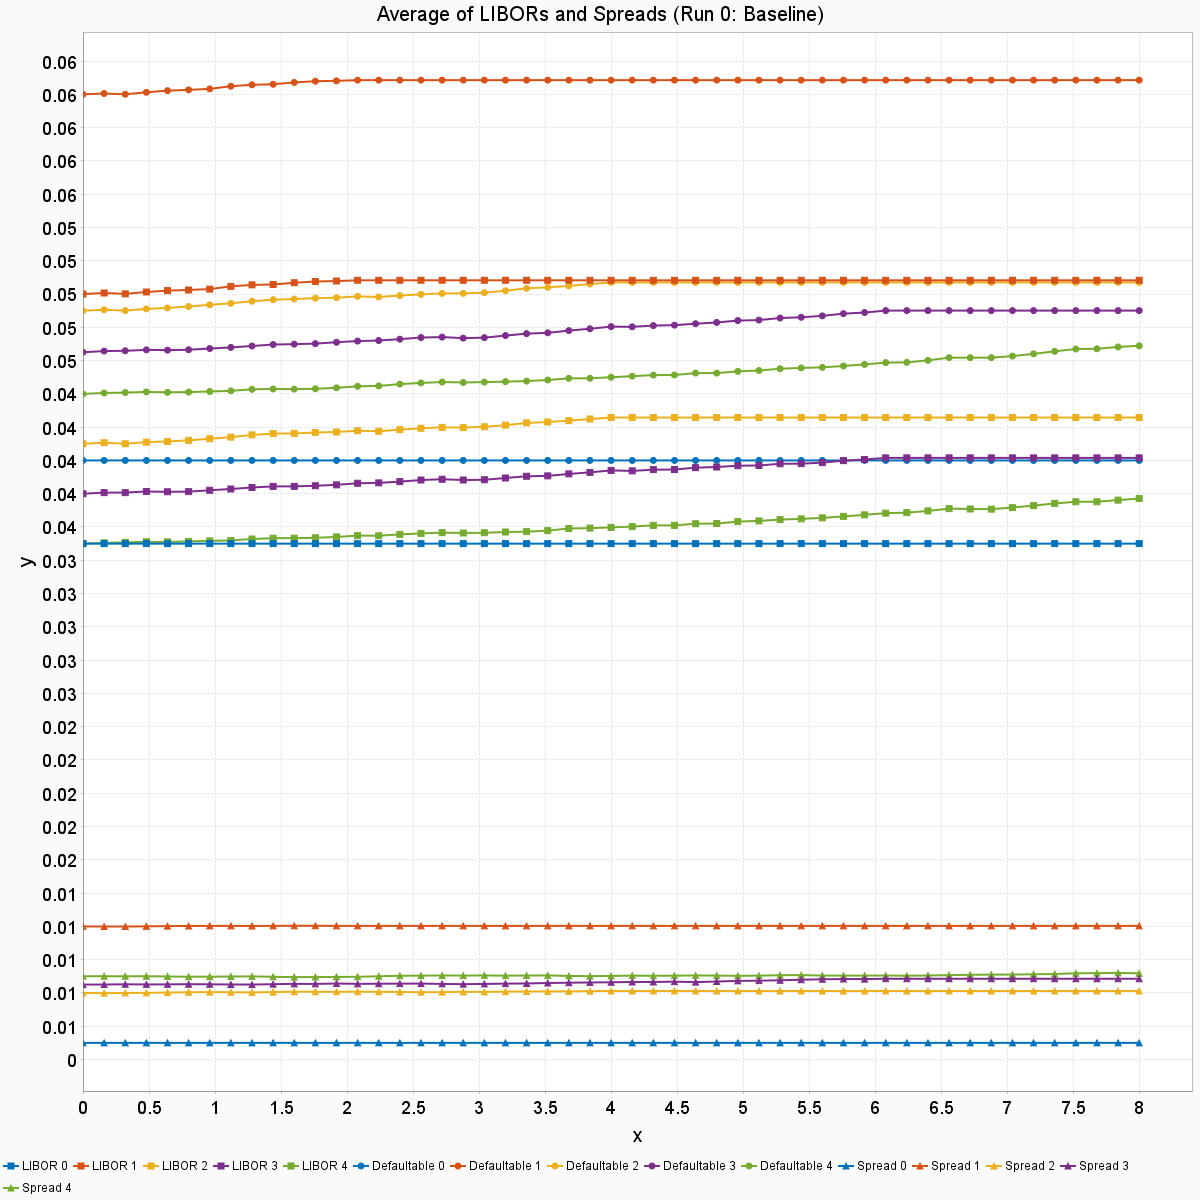
\includegraphics[height=0.6\textheight]{VorstellungPics/FreeParamsRange05}
		\caption[]{Averages of LIBORs and Spreads for $f_{i k} \in [-0.5, 0.5]$}
		\label{fig:freeparamsrange05}
	\end{figure}
	
		
	\end{frame}
	
	\begin{frame}
	\frametitle{Results}
	\begin{figure}
		\centering
		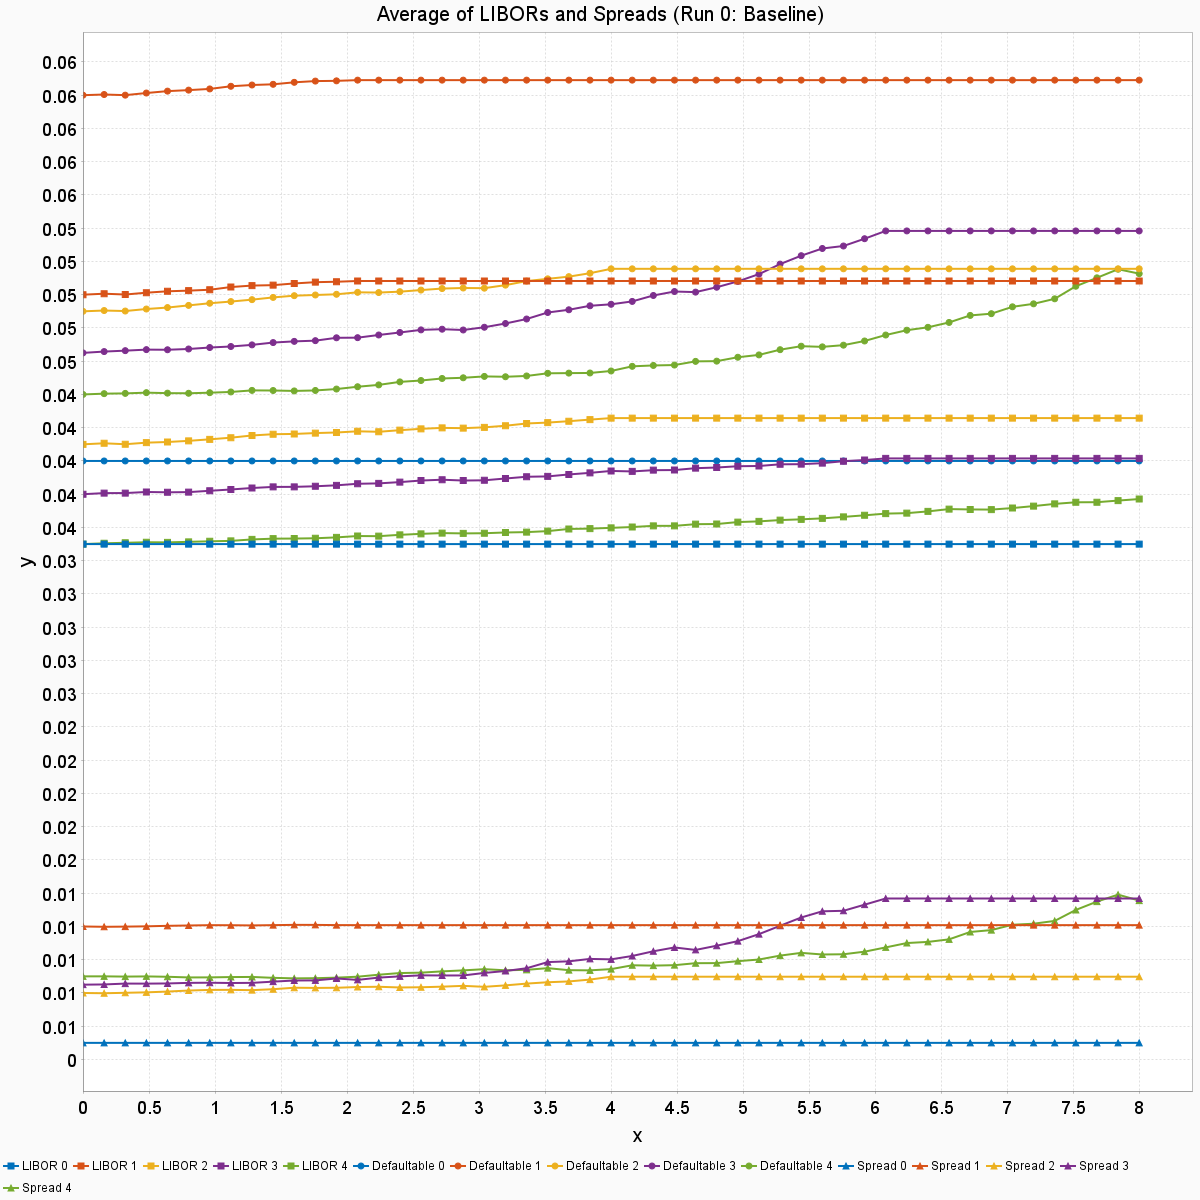
\includegraphics[height=0.6\textheight]{VorstellungPics/FreeParamsRange10}
		\caption[]{Averages of LIBORs and Spreads for $f_{i k} \in [-1.0, 1.0]$}
		\label{fig:freeparamsrange10}
	\end{figure}
	
	\end{frame}
	
	\begin{frame}
		\frametitle{Results}
		\begin{figure}
			\centering
			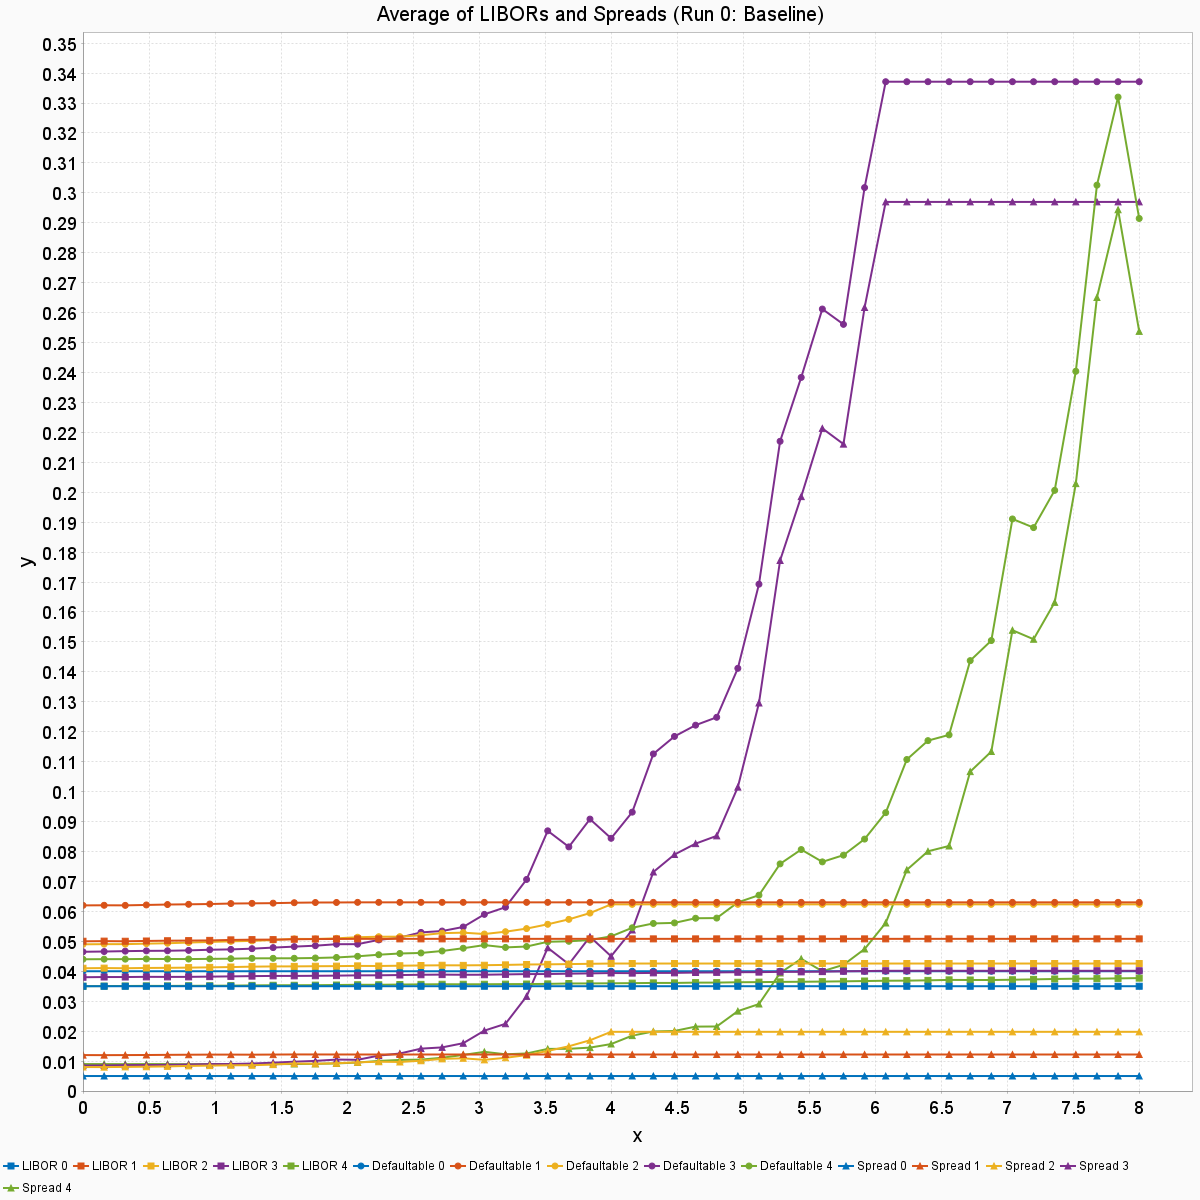
\includegraphics[height=0.6\textheight]{VorstellungPics/FreeParamsRange15}
			\caption[]{Averages of LIBORs and Spreads for $f_{i k} \in [-1.5, 1.5]$}
			\label{fig:freeparamsrange15}
		\end{figure}
		
		
	\end{frame}
	
	\section{Loan Pricing}\label{sectLoans}
	
	\begin{frame}
	\frametitle{\nameref{sectLoans}}
	\tableofcontents[ 
	currentsection, 
	sectionstyle=show/shaded, 
	subsectionstyle=show/shaded, 
	] 
	\end{frame}
	
	\begin{frame}
		\frametitle{Pricing claims}
		To price claims with this model we apply the default probability to those parts of the claim, that are dependent on survival.\\
		
		E.g. a $T_i$ claim which is fully conditional on the survival of the modeled entity has the price:
		\[
		B(0)\mathbb{E}^{\mathbb{Q}^B}\left[\frac{X^d}{B(T_i)}\right] = B(0)\mathbb{E}^{\mathbb{Q}^B}\left[\frac{X}{B(T_i)}\mathbb{Q}^B(\tau > T_i)\right],
		\]
		where $X^d$ is the claim, and $X$ is the claim if the entity would have no default probability.\\
		An application for this are loan related options.
	\end{frame}
	
	\begin{frame}
		\frametitle{Simple Loans}
		A loan is nothing else than a defaultable coupon bond issued by the debtor.\\
		The price of a defaultable coupon bond with nominal \(N\) and coupons \(c_i\) paid at $\tilde{T}_i \in \{T_1, ..., T_N\}$ is:
		\[C^d(t) = \sum_{i=1}^{M}c_iP^d(t;\tilde{T}_i),\]
		for $t\in [0, \tilde{T}_1]$. Pricing the loan comes down to establishing the coupon rates such that the initial price of the coupon bond is equal to the nominal:
		\[N \mbeq \sum_{i=1}^{M}c_i P^d(0;\tilde{T}_i)\]
		Note: if the loan is not an amortizing one $c_M = N + \tilde{c}_M$.
	\end{frame}
	
	\begin{frame}
		\frametitle{Cancellable Loans}
		A cancellable loan is a loan that can be canceled (payed back completely) at - in this simple example - a fixed time \(T_k \in \{T_1, ..., T_{M-1}\}\):
		\begin{figure}
			\centering
			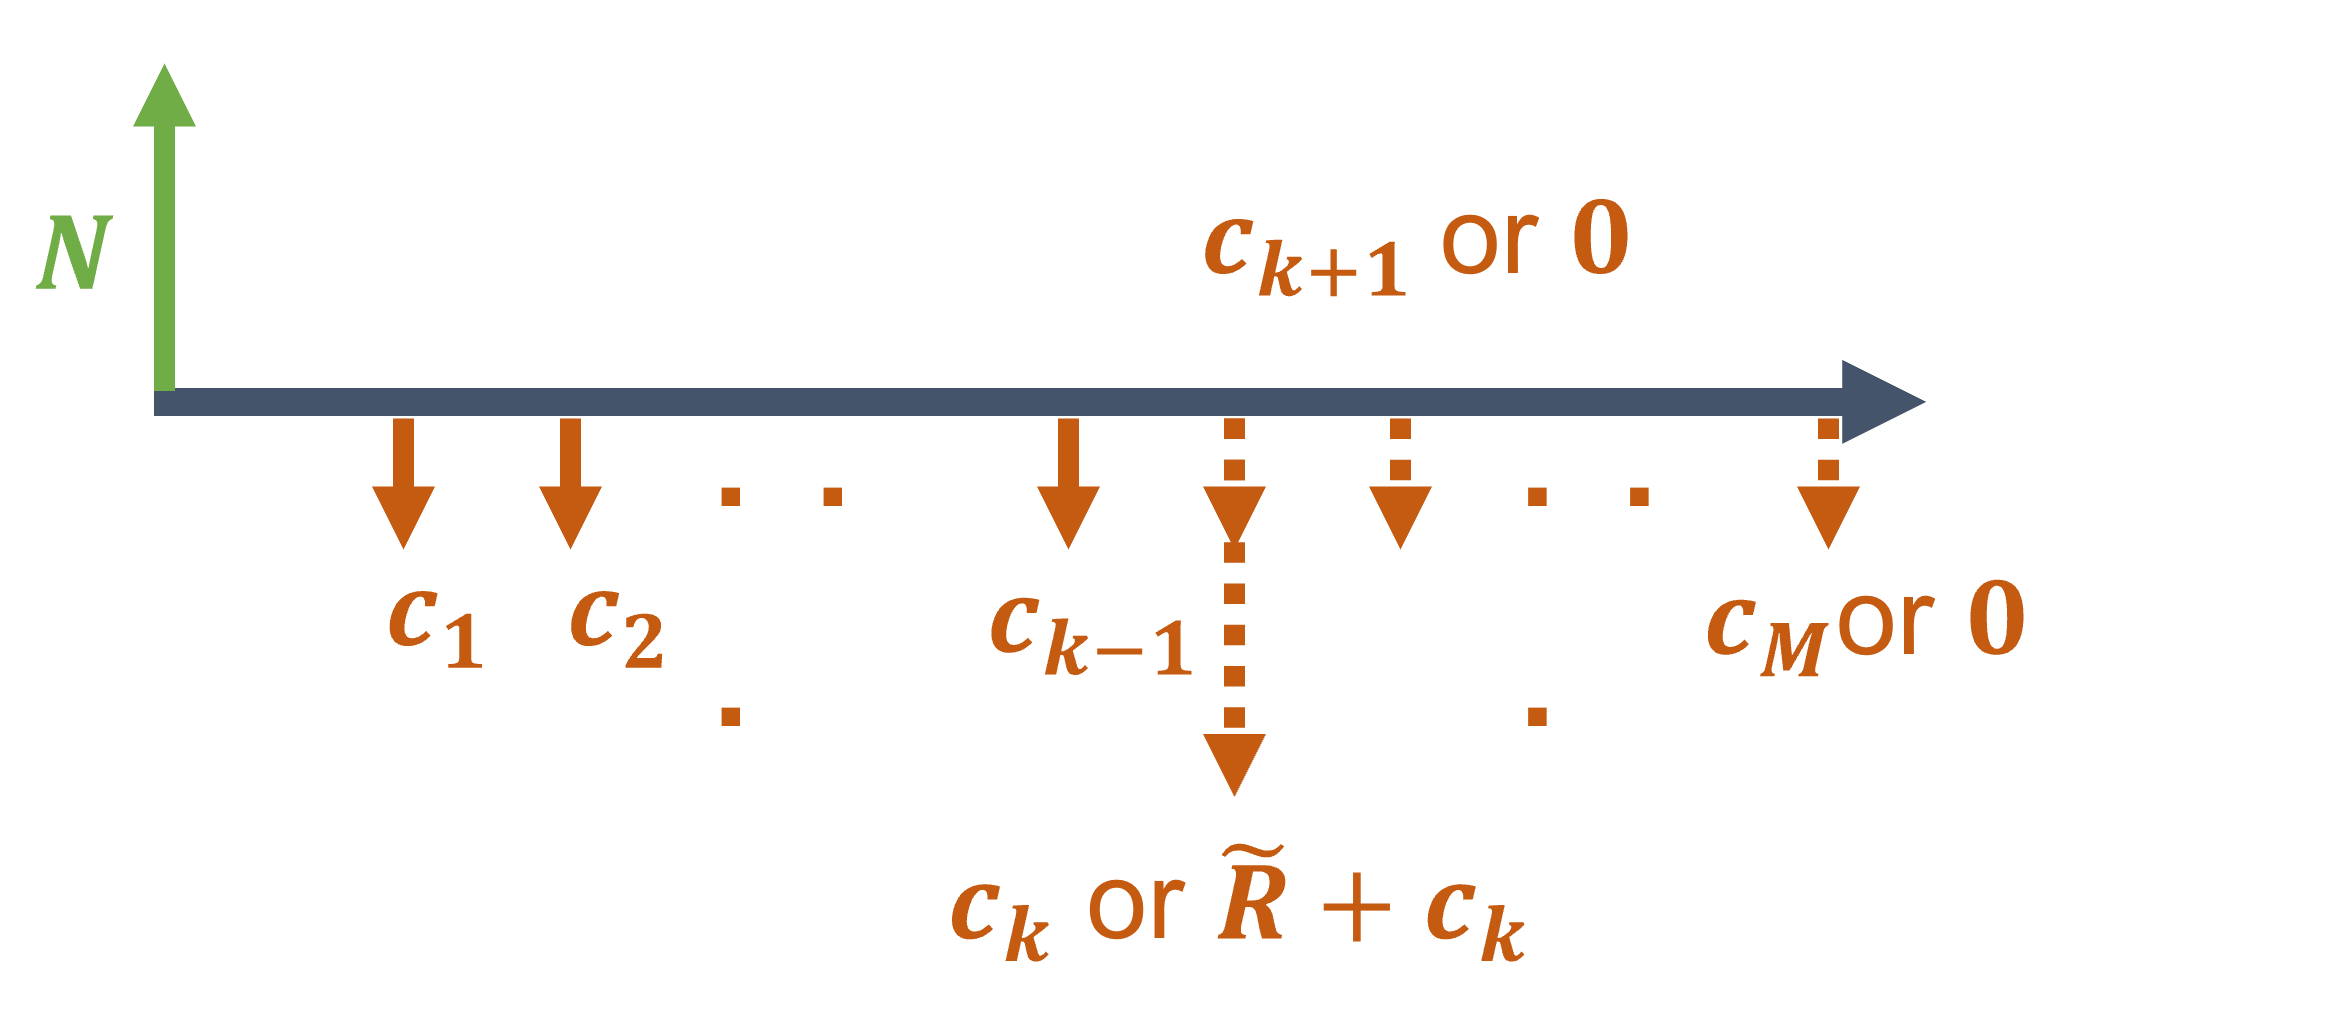
\includegraphics[width=0.5\linewidth]{CancellableLoan}
			\caption[Cashflow of a cancellable loan]{Cashflow of a cancellable loan}
			\label{fig:cancellableLoan}
		\end{figure}
		where \(\tilde{R} = \dfrac{\sum_{i=k+1}^{M}c_i P^d(0;T_i)}{P^d(0;T_k)}\) is the redemption of the loan.
		
	\end{frame}
	
	\begin{frame}
		\frametitle{Cancellable Loans}
	We can derive a price formula by splitting the definite loan and the optional part:
		\begin{figure}
			\centering
			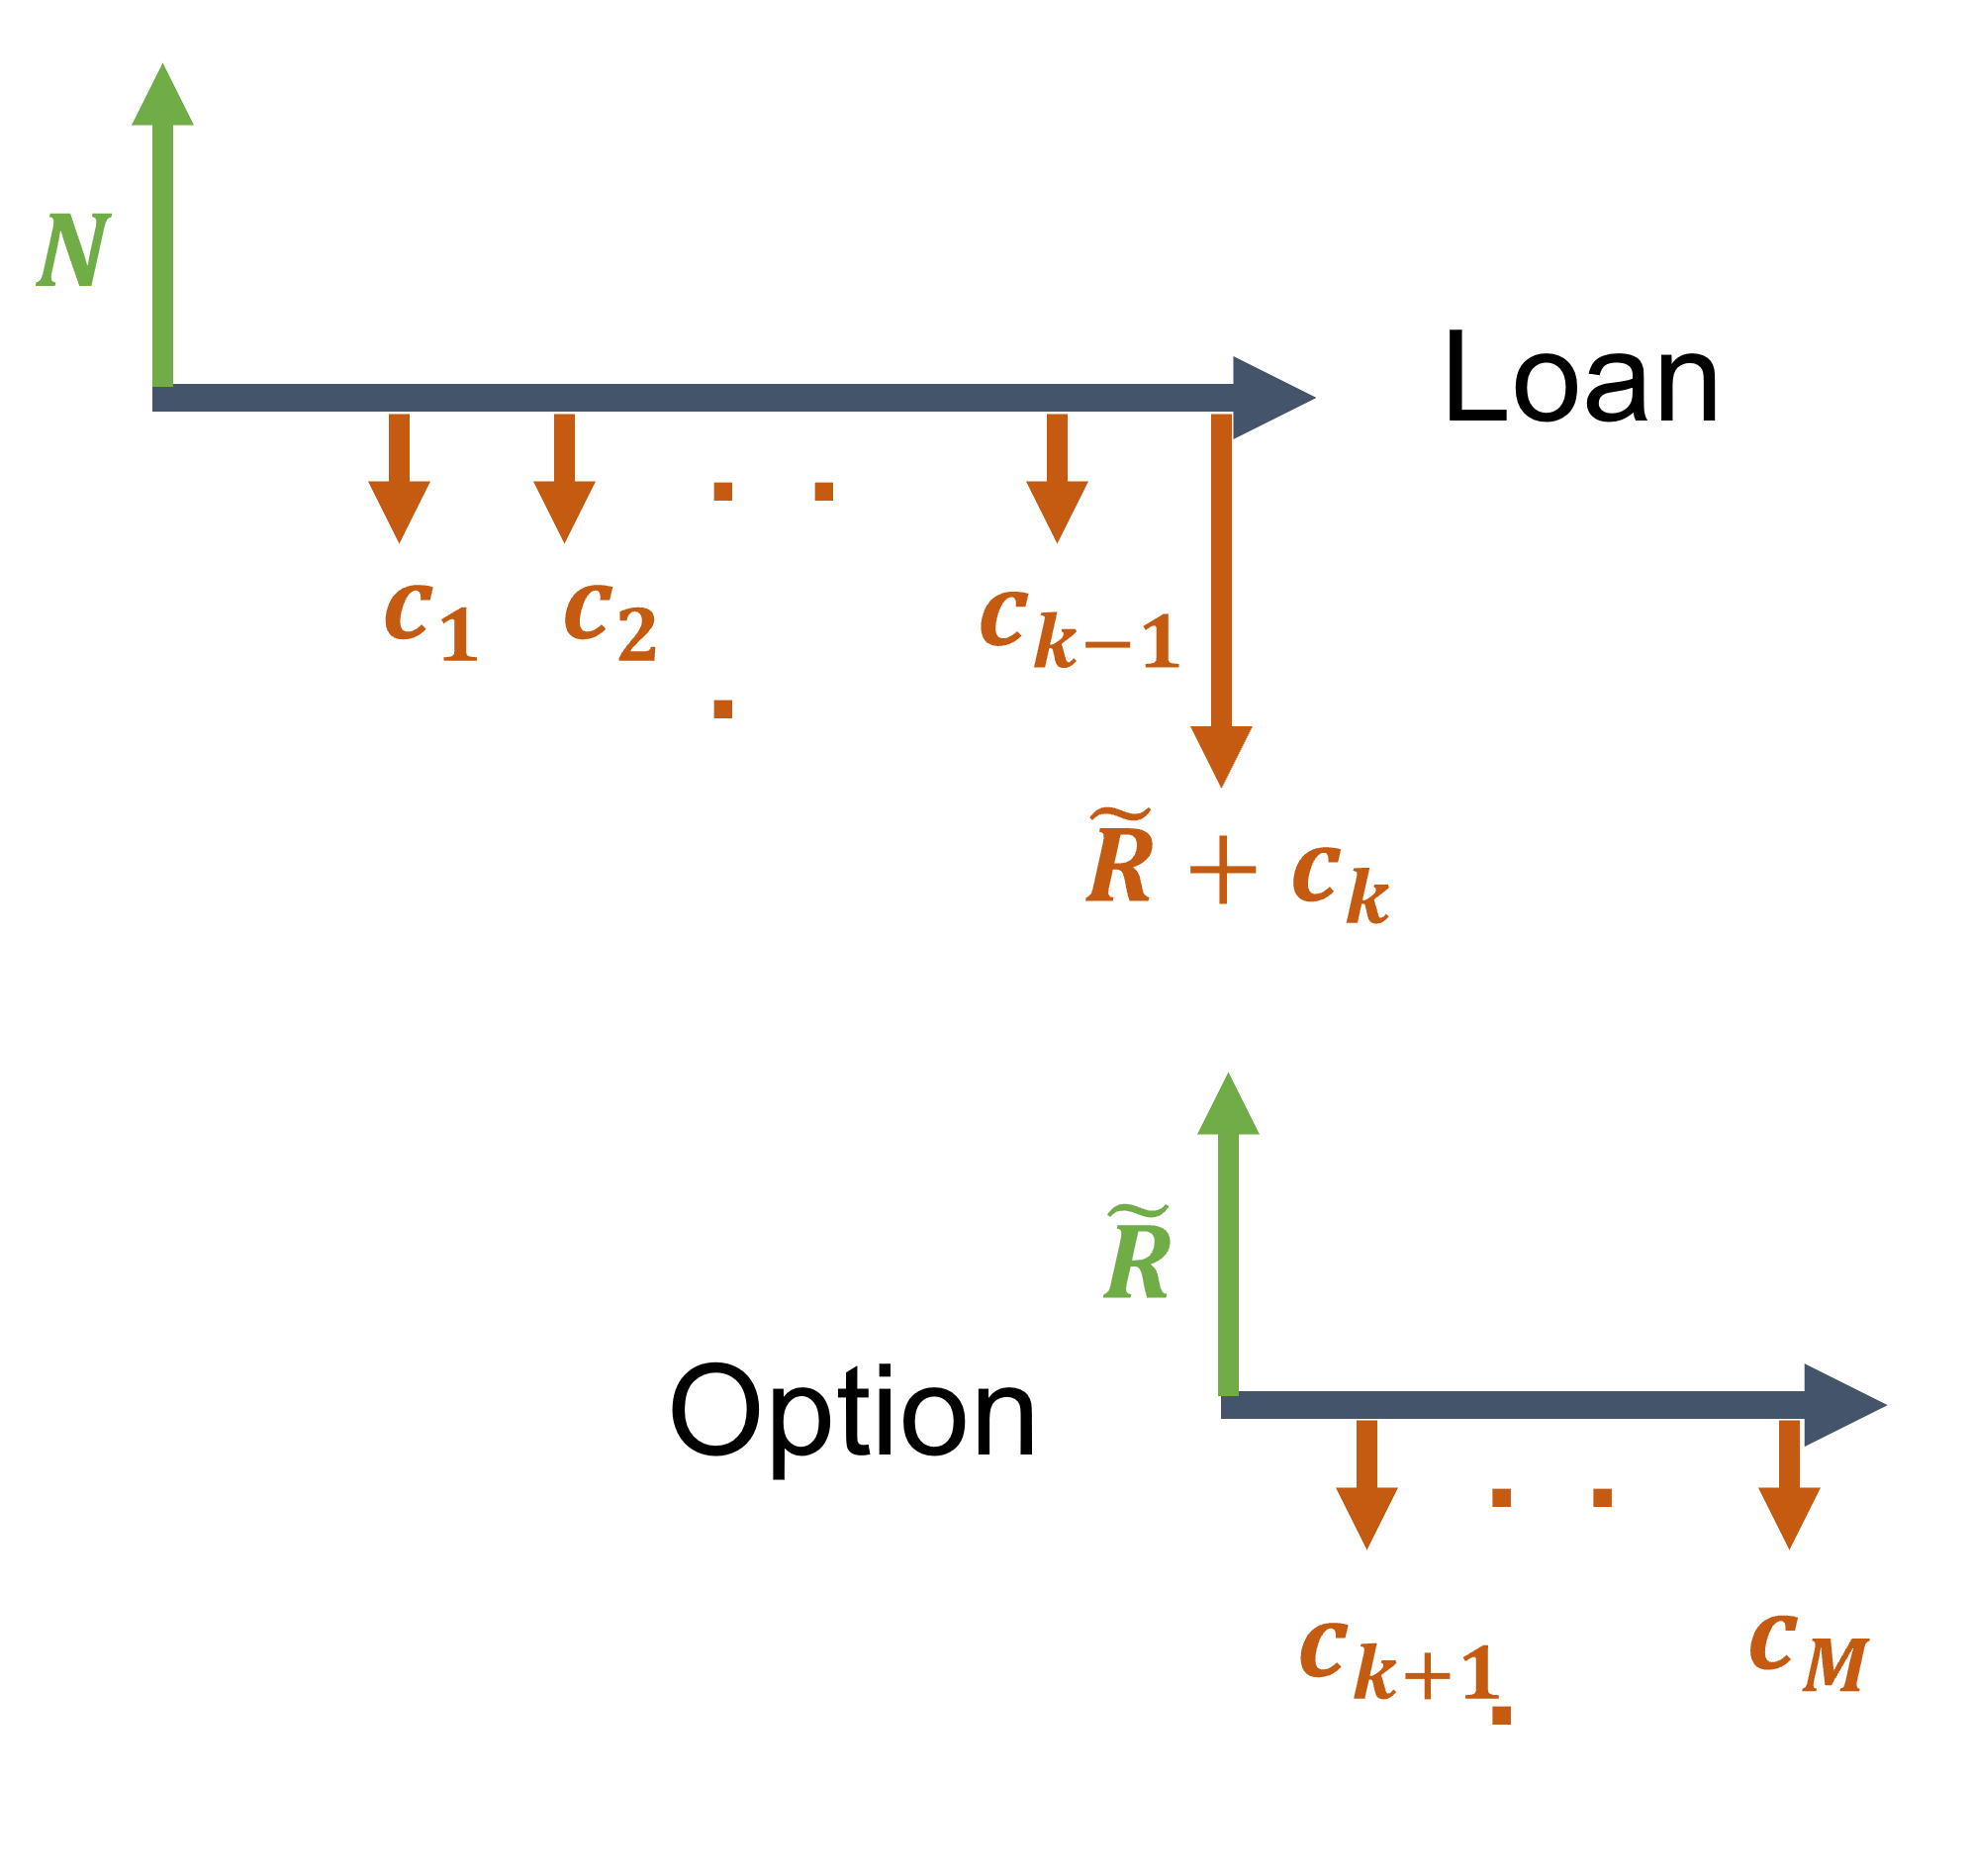
\includegraphics[height=150pt]{LoanAndOption}
			\caption[Splitted Cashflow of a cancellable loan]{Cashflow of a cancellable loan}
			\label{fig:loanAndOption}
		\end{figure}
		
		
	\end{frame}
	
	\begin{frame}
		\frametitle{Cancellable Loans}
		Hence the option is a European put option with strike price \(\tilde{R}\) on a coupon bond with coupons \(c_{k+1}, ..., c_{M}\) and nominal \(\tilde{R}\). In other words the debtor has the right (but not the obligation) to enter a second loan for the conditions of today.\\
		This yields an adjustment in the derivation of the coupons:
		\[N + V^P(0) \mbeq \sum_{i=1}^{M}c_i P^d(0;T_i)\]
		where \[V^P(t) = B(t)\mathbb{E}^{\mathbb{Q}^B}\left[\left.\frac{(\tilde{R} - C^d(T_k))^+}{B(T_k)} \mathbb{Q}^B(\tau > T_k | \tau > t)\; \right| \;\mathcal{F}_t\right]\]
		\end{frame}
	
	\begin{frame}
		\frametitle{What's next?}
		\begin{itemize}
			\item Deriving more complicated products like loans that can be canceled at any tenor.
			\item Constructing products, where both counterparties are defaultable: the issuer and the buyer.
			\item Construct products, where the decision to cancel the loan is flawed.
		\end{itemize}
	\end{frame}
	
	\section{Bibliography}
	
	\begin{frame}{Bibliography}
		\tiny
		\bibliographystyle{acm}
		\bibliography{Bibliographie}
	\end{frame}
\end{document}